% =============================================================================
% PART B - MODULES 24-26: MILESTONES, FILES & SUBMISSIONS
%   (UC-24.01 - UC-24.06, UC-25.01 - UC-25.03, UC-26.01 - UC-26.05)
% In Charge: Vo Nhut Tin (CE180619)
% =============================================================================

\newpage
\subsection{Modules 24--26: Milestones, Shared Files \& Deliverable Submissions}

This suite of modules enables Clients and Freelancers to organize project execution into verifiable delivery stages (\textit{Milestones}), exchange milestone-specific working files, start active execution, submit deliverables with preview links and archives, request targeted revisions, and release escrow funds upon approval.

% -----------------------------------------------------------------------------
\subsubsection{M24.01 -- View Milestones List (UC-24.01)}

\begin{itemize}[leftmargin=1.5em,itemsep=2pt]
  \item \textbf{Screen Name \& Route Path:} Milestones Timeline Screen -- \texttt{/[role]/\allowbreak{}contracts/\allowbreak{}[slug]/\allowbreak{}milestones}.
  \item \textbf{Target Actor:} Client, Freelancer.
  \item \Needspace{6\baselineskip}\textbf{Before You Begin:} Contract exists and you navigate to its \textbf{Milestones} view via the header breadcrumb.
\end{itemize}
\begin{figure}[H]\centering
  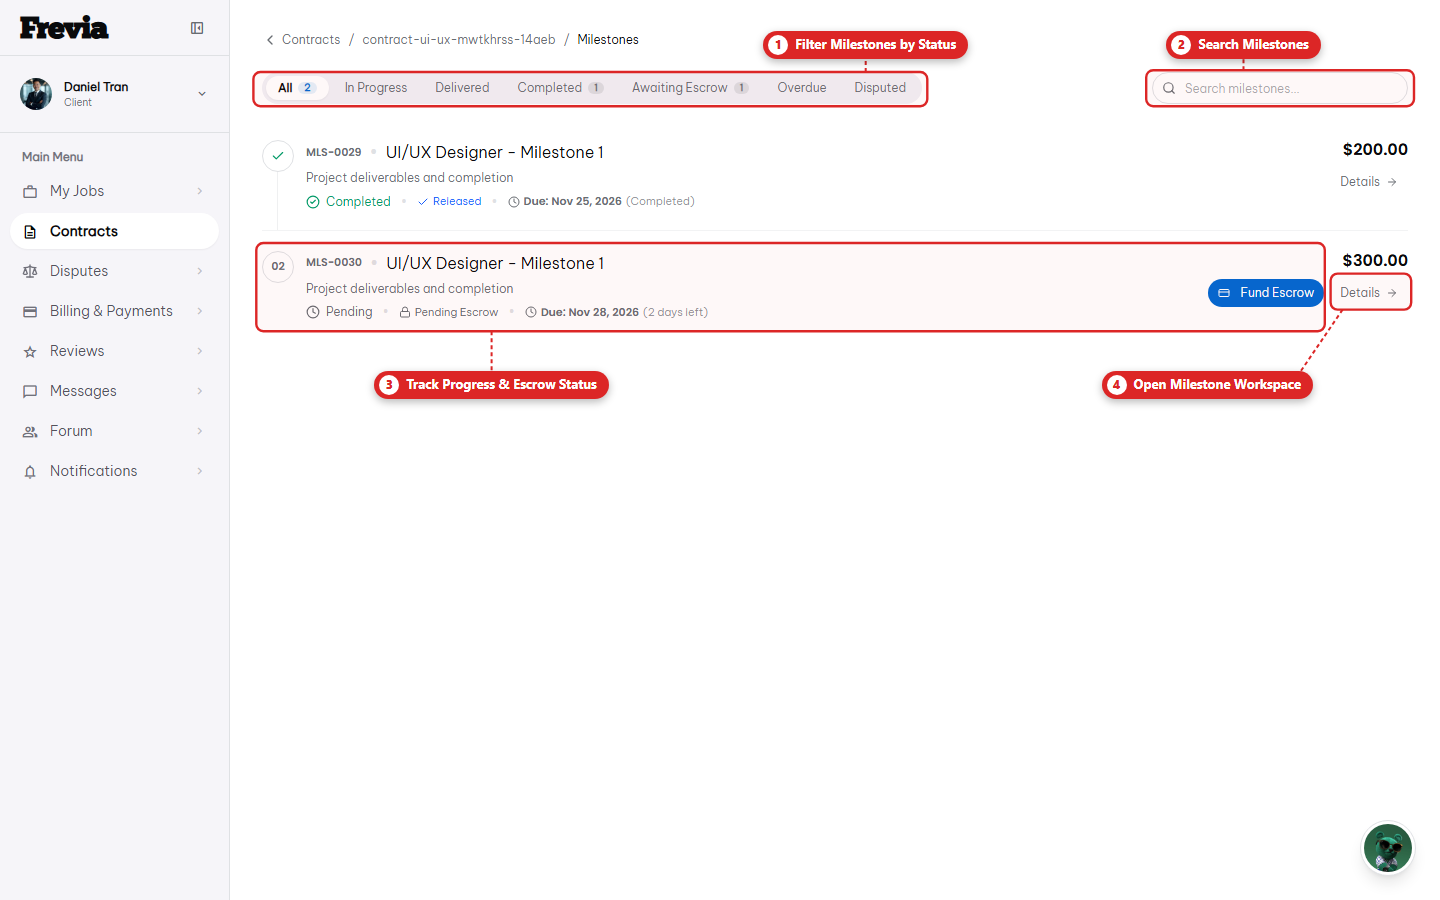
\includegraphics[width=0.90\textwidth]{images/milestones/m24_01_view_milestone_list_guide.png}
  \caption{Contract Milestones list with status filter tabs, search, and escrow actions}
  \label{fig:m24_01_view_milestone_list}
\end{figure}
\Needspace{6\baselineskip}\paragraph{Step-by-Step User Guide:}
\begin{enumerate}[leftmargin=1.8em,itemsep=3pt]
  \item \rbadge{1} \textbf{Filter Milestones by Status:} Click status pills (\textbf{All}, \textbf{In Progress}, \textbf{Delivered}, \textbf{Completed}, \textbf{Awaiting Escrow}, \textbf{Overdue}, \textbf{Disputed}).
  \item \rbadge{2} \textbf{Search Milestones:} Enter a milestone title or ID in \textit{Search milestones...} to filter rows instantaneously.
  \item \rbadge{3} \textbf{Track Progress \& Escrow Status:} Inspect payment badges (\textit{Pending Escrow}, \textit{Escrow Funded}, \textit{Released}), due-date countdowns, and inline \textbf{Fund Escrow} buttons.
  \item \rbadge{4} \textbf{Open Milestone Workspace:} Click \textbf{Details $\rightarrow$} on any milestone row to open its full multi-tab workspace.
\end{enumerate}
\Needspace{6\baselineskip}\paragraph{After You Submit (Result \& Troubleshooting):}
\begin{itemize}[leftmargin=1.5em,itemsep=2pt]
  \item \textbf{What Happens Next:} All contract milestones appear in sequential order with real-time payment and delivery status indicators.
  \item \textbf{Troubleshooting \& Common Messages:} Overdue unfunded or undelivered milestones past due date automatically highlight an \textit{Overdue (Late)} indicator.
\end{itemize}

% -----------------------------------------------------------------------------
\newpage
\subsubsection{M24.02 -- View Milestone Details (UC-24.02)}

\begin{itemize}[leftmargin=1.5em,itemsep=2pt]
  \item \textbf{Screen Name \& Route Path:} Milestone Detail Workspace -- \texttt{/[role]/\allowbreak{}contracts/\allowbreak{}[slug]/\allowbreak{}milestones/\allowbreak{}[milestoneId]}.
  \item \textbf{Target Actor:} Client, Freelancer.
  \item \Needspace{6\baselineskip}\textbf{Before You Begin:} Select a milestone from the contract's Milestones list.
\end{itemize}
\begin{figure}[H]\centering
  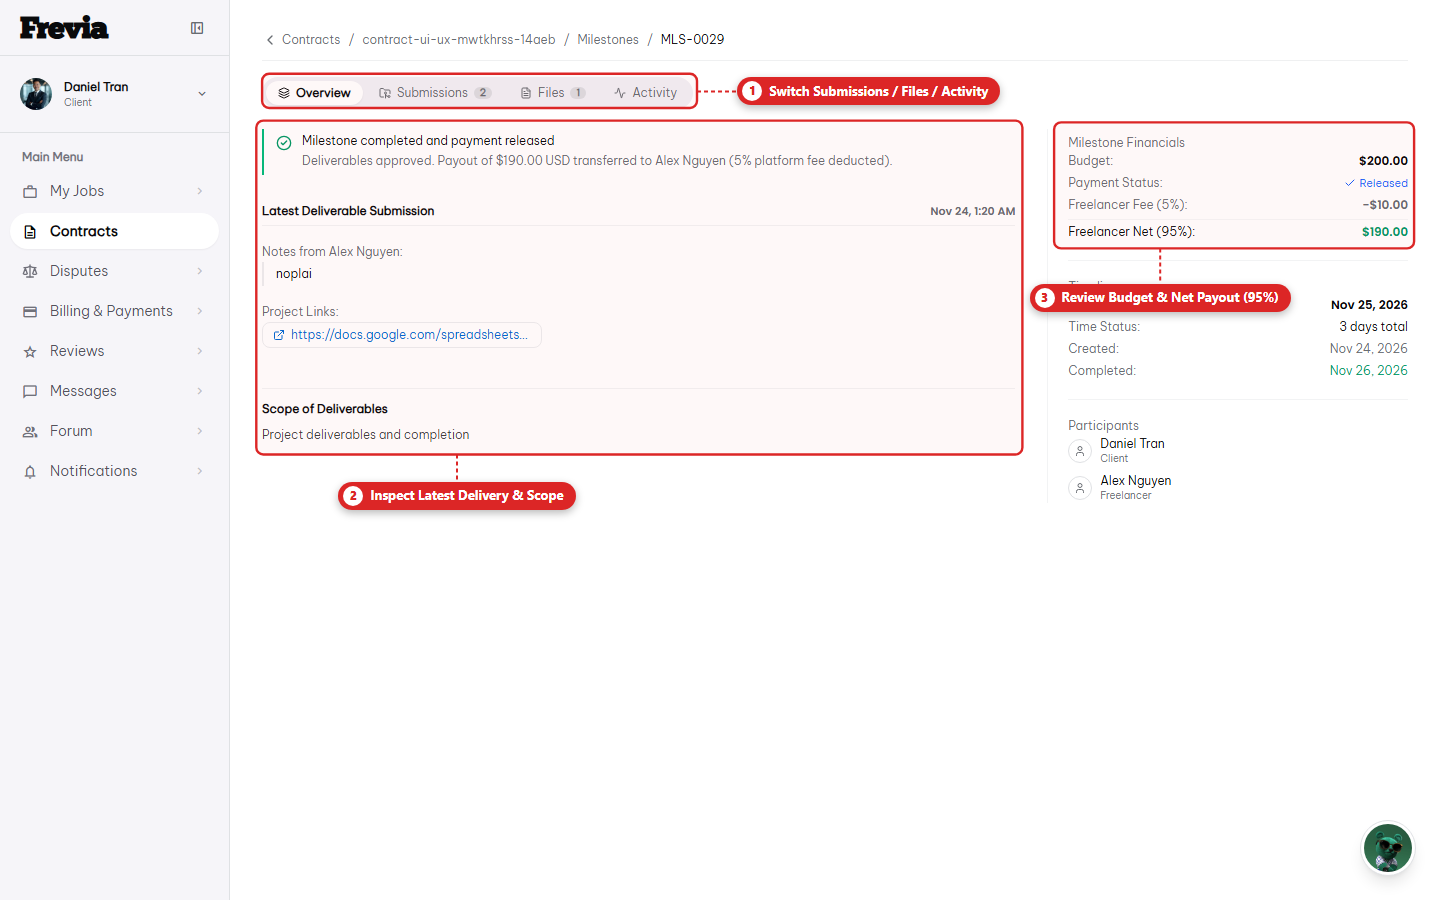
\includegraphics[width=0.90\textwidth]{images/milestones/m24_02_view_milestone_detail_guide.png}
  \caption{Milestone detail workspace displaying tabs, latest delivery, and 95\% net financials}
  \label{fig:m24_02_view_milestone_detail}
\end{figure}
\Needspace{6\baselineskip}\paragraph{Step-by-Step User Guide:}
\begin{enumerate}[leftmargin=1.8em,itemsep=3pt]
  \item \rbadge{1} \textbf{Switch Submissions / Files / Activity:} Use the segmented tab bar at top to switch between \textbf{Overview}, \textbf{Submissions}, \textbf{Files}, and \textbf{Activity}.
  \item \rbadge{2} \textbf{Inspect Latest Delivery \& Scope:} Read the completion banner, latest freelancer notes, verification links, and deliverable scope requirements.
  \item \rbadge{3} \textbf{Review Budget \& Net Payout (95\%):} Check the right-hand \textbf{Milestone Financials} sidebar showing gross budget, 5\% freelancer platform fee, net payout, timeline, and participants.
\end{enumerate}
\Needspace{6\baselineskip}\paragraph{After You Submit (Result \& Troubleshooting):}
\begin{itemize}[leftmargin=1.5em,itemsep=2pt]
  \item \textbf{What Happens Next:} Full milestone context, financial breakdown, and current status actions synchronize dynamically.
  \item \textbf{Troubleshooting \& Common Messages:} Accessing an invalid or unauthorized milestone ID renders a clean 404 or 403 boundary page.
\end{itemize}

% -----------------------------------------------------------------------------
\newpage
\subsubsection{M24.03 -- Create Milestone (UC-24.03)}

\begin{itemize}[leftmargin=1.5em,itemsep=2pt]
  \item \textbf{Screen Name \& Route Path:} Add New Milestone Drawer -- \texttt{/client/\allowbreak{}contracts/\allowbreak{}[slug]}.
  \item \textbf{Target Actor:} Client.
  \item \Needspace{6\baselineskip}\textbf{Before You Begin:} Contract is editable with unallocated budget available (click \textbf{+ Add Milestone} inside Section 3 or the Milestones page).
\end{itemize}
\begin{figure}[H]\centering
  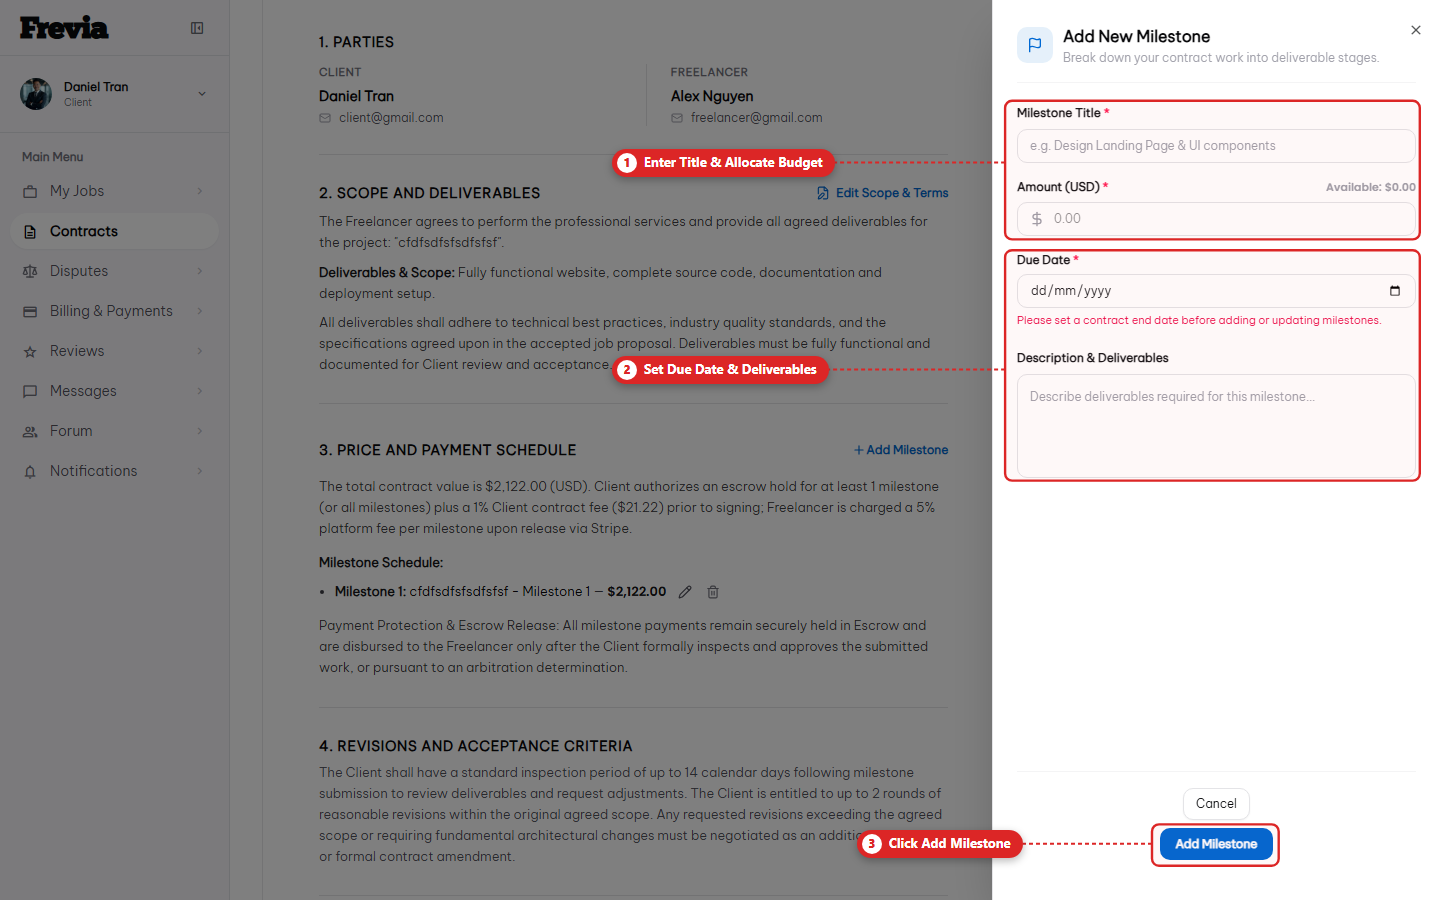
\includegraphics[width=0.90\textwidth]{images/milestones/m24_03_create_milestone_guide.png}
  \caption{Add New Milestone slide-over drawer with unallocated budget check}
  \label{fig:m24_03_create_milestone}
\end{figure}
\Needspace{6\baselineskip}\paragraph{Step-by-Step User Guide:}
\begin{enumerate}[leftmargin=1.8em,itemsep=3pt]
  \item \rbadge{1} \textbf{Enter Title \& Allocate Budget:} Provide a descriptive \textit{Milestone Title} and specify \textit{Amount (USD)} without exceeding the displayed \textit{Available} balance.
  \item \rbadge{2} \textbf{Set Due Date \& Deliverables:} Choose a valid future \textit{Due Date} within the Contract End Date and describe required deliverables.
  \item \rbadge{3} \textbf{Click Add Milestone:} Click the blue \textbf{Add Milestone} button to append the stage to the contract schedule.
\end{enumerate}
\Needspace{6\baselineskip}\paragraph{After You Submit (Result \& Troubleshooting):}
\begin{itemize}[leftmargin=1.5em,itemsep=2pt]
  \item \textbf{What Happens Next:} The milestone saves in \texttt{PENDING} status (\textit{Pending Escrow}) and updates the contract's Price and Payment Schedule.
  \item \textbf{Troubleshooting \& Common Messages:} If the Contract End Date has not been set yet, an inline reminder asks you to configure the Contract End Date first.
\end{itemize}

% -----------------------------------------------------------------------------
\newpage
\subsubsection{M24.04 -- Update Milestone (UC-24.04)}

\begin{itemize}[leftmargin=1.5em,itemsep=2pt]
  \item \textbf{Screen Name \& Route Path:} Edit Milestone Drawer -- \texttt{/client/\allowbreak{}contracts/\allowbreak{}[slug]/\allowbreak{}milestones}.
  \item \textbf{Target Actor:} Client.
  \item \Needspace{6\baselineskip}\textbf{Before You Begin:} Click the pencil edit icon on an unfunded or uncompleted milestone row.
\end{itemize}
\begin{figure}[H]\centering
  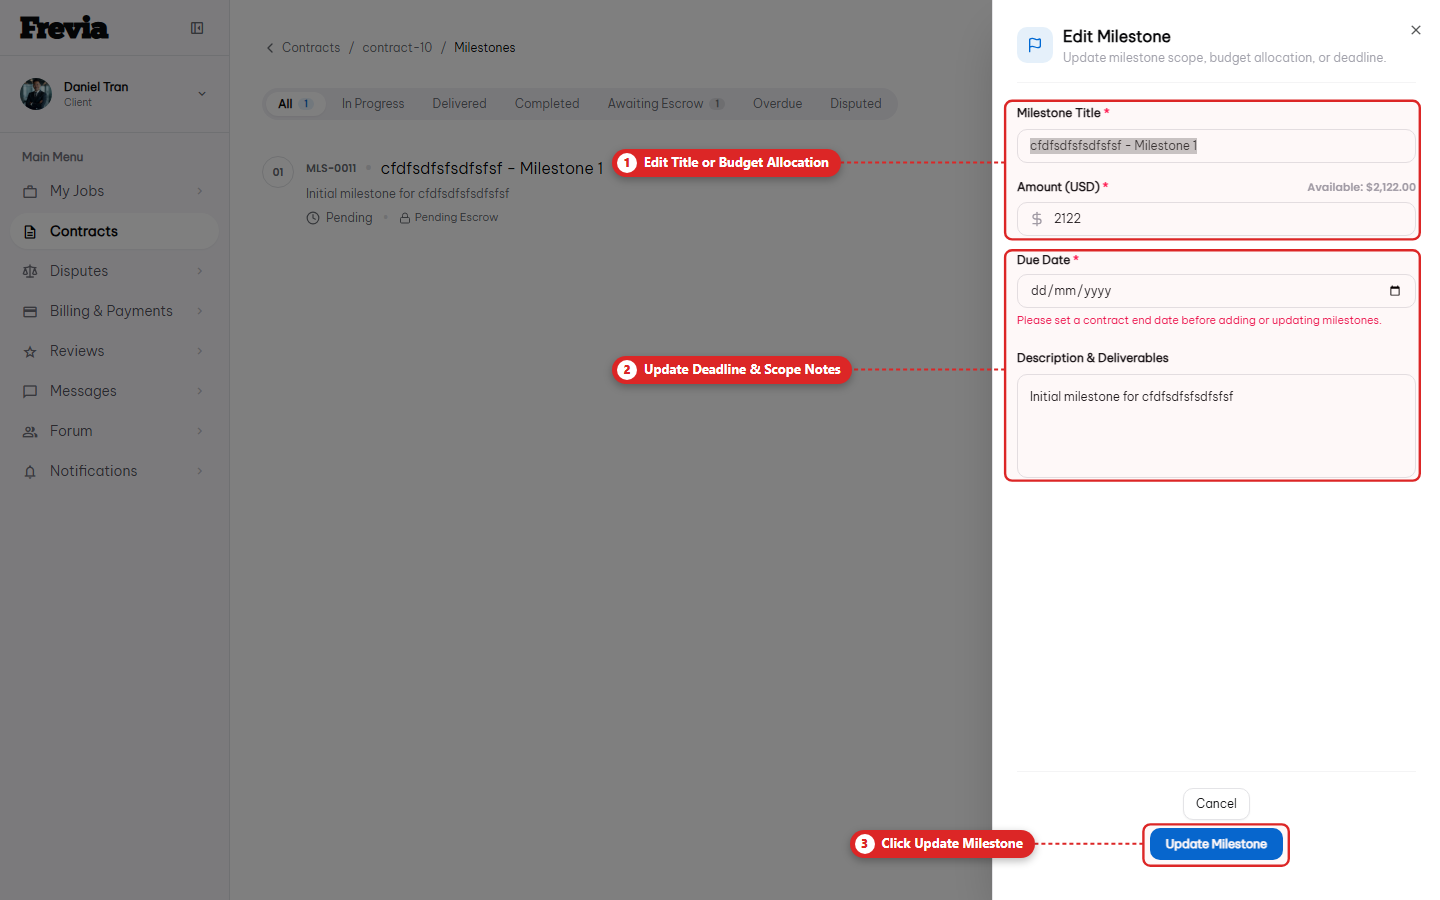
\includegraphics[width=0.90\textwidth]{images/milestones/m24_04_update_milestone_guide.png}
  \caption{Edit Milestone drawer for updating scope, amount, and deadline}
  \label{fig:m24_04_update_milestone}
\end{figure}
\Needspace{6\baselineskip}\paragraph{Step-by-Step User Guide:}
\begin{enumerate}[leftmargin=1.8em,itemsep=3pt]
  \item \rbadge{1} \textbf{Edit Title or Budget Allocation:} Adjust \textit{Milestone Title} or revise \textit{Amount (USD)} within the remaining unallocated pool.
  \item \rbadge{2} \textbf{Update Deadline \& Scope Notes:} Modify \textit{Due Date} or refine \textit{Description \& Deliverables}.
  \item \rbadge{3} \textbf{Click Update Milestone:} Click \textbf{Update Milestone} to save changes immediately.
\end{enumerate}
\Needspace{6\baselineskip}\paragraph{After You Submit (Result \& Troubleshooting):}
\begin{itemize}[leftmargin=1.5em,itemsep=2pt]
  \item \textbf{What Happens Next:} Updated milestone amounts, titles, and due dates propagate across both Contract Detail and Milestones tabs.
  \item \textbf{Troubleshooting \& Common Messages:} Funded or completed milestone amounts are locked against reduction after escrow authorization.
\end{itemize}

% -----------------------------------------------------------------------------
\newpage
\subsubsection{M24.05 -- Delete Milestone (UC-24.05)}

\begin{itemize}[leftmargin=1.5em,itemsep=2pt]
  \item \textbf{Screen Name \& Route Path:} Delete Milestone Modal -- \texttt{/client/\allowbreak{}contracts/\allowbreak{}[slug]/\allowbreak{}milestones}.
  \item \textbf{Target Actor:} Client.
  \item \Needspace{6\baselineskip}\textbf{Before You Begin:} Click the trash icon on an unfunded milestone (\texttt{paymentStatus = PENDING}).
\end{itemize}
\begin{figure}[H]\centering
  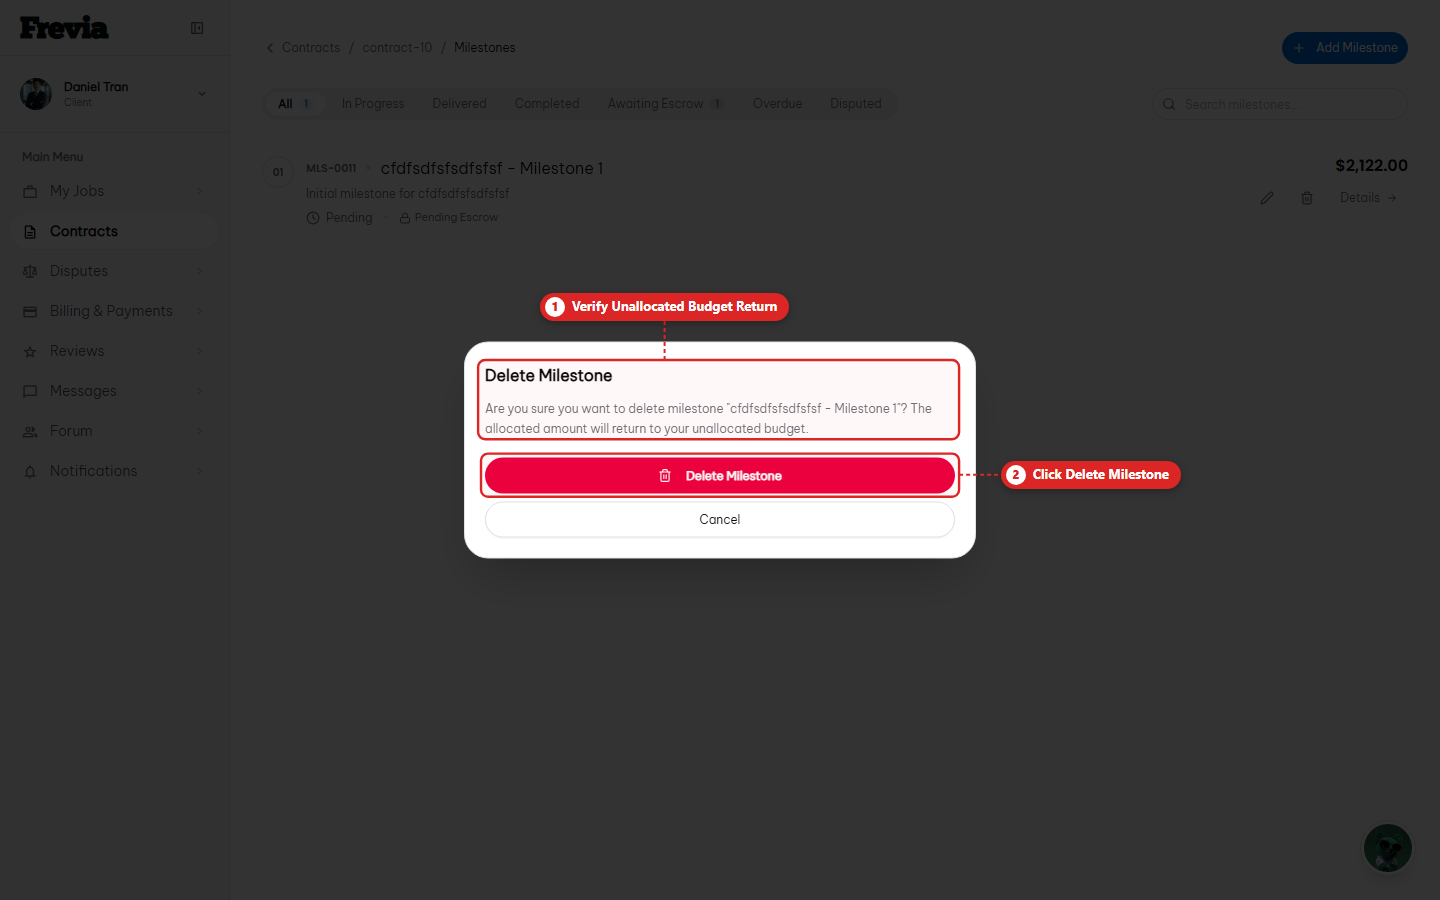
\includegraphics[width=0.90\textwidth]{images/milestones/m24_05_delete_milestone_guide.png}
  \caption{Delete Milestone confirmation modal showing budget reallocation}
  \label{fig:m24_05_delete_milestone}
\end{figure}
\Needspace{6\baselineskip}\paragraph{Step-by-Step User Guide:}
\begin{enumerate}[leftmargin=1.8em,itemsep=3pt]
  \item \rbadge{1} \textbf{Verify Unallocated Budget Return:} Review the milestone name and confirmation note explaining that its budget will return to your unallocated contract pool.
  \item \rbadge{2} \textbf{Click Delete Milestone:} Click the red \textbf{Delete Milestone} button to delete the stage permanently.
\end{enumerate}
\Needspace{6\baselineskip}\paragraph{After You Submit (Result \& Troubleshooting):}
\begin{itemize}[leftmargin=1.5em,itemsep=2pt]
  \item \textbf{What Happens Next:} The milestone disappears from the schedule and its budget becomes available for creating or resizing other milestones.
  \item \textbf{Troubleshooting \& Common Messages:} Funded (\texttt{FUNDED}) or completed milestones cannot be deleted directly (\textit{MilestoneCannotBeDeleted}).
\end{itemize}

% -----------------------------------------------------------------------------
\newpage
\subsubsection{M24.06 -- Update Milestone Progress (UC-24.06)}

\begin{itemize}[leftmargin=1.5em,itemsep=2pt]
  \item \textbf{Screen Name \& Route Path:} Freelancer Milestones Workspace -- \texttt{/freelancer/\allowbreak{}contracts/\allowbreak{}[slug]/\allowbreak{}milestones}.
  \item \textbf{Target Actor:} Freelancer.
  \item \Needspace{6\baselineskip}\textbf{Before You Begin:} The milestone is \texttt{Escrow Funded} and the contract is \texttt{ACTIVE}.
\end{itemize}
\begin{figure}[H]\centering
  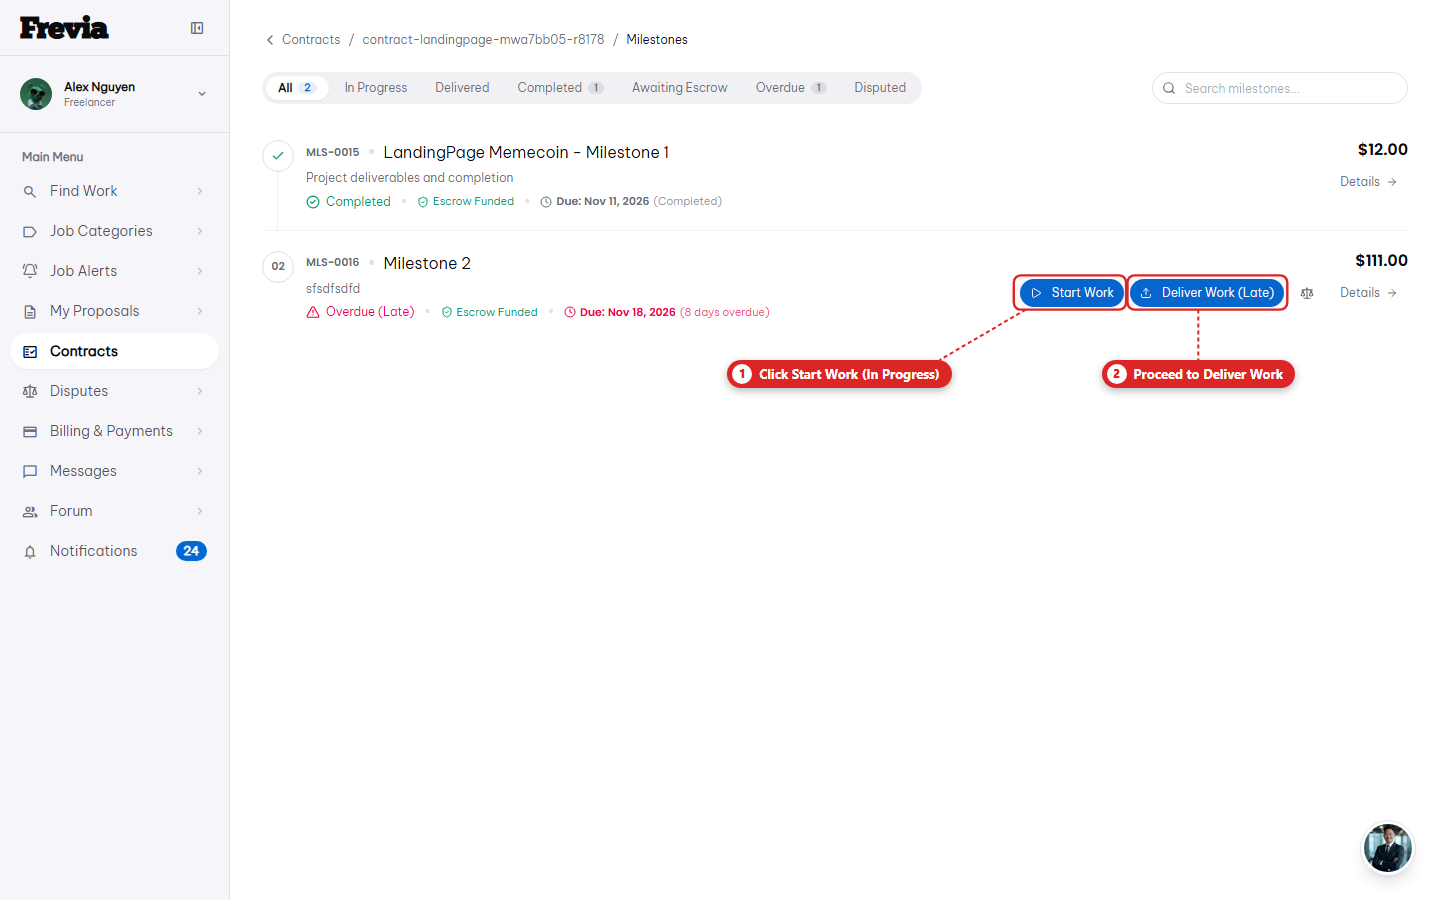
\includegraphics[width=0.90\textwidth]{images/milestones/m24_06_update_milestone_progress_guide.png}
  \caption{Freelancer advancing a funded milestone to In Progress via Start Work}
  \label{fig:m24_06_update_milestone_progress}
\end{figure}
\Needspace{6\baselineskip}\paragraph{Step-by-Step User Guide:}
\begin{enumerate}[leftmargin=1.8em,itemsep=3pt]
  \item \rbadge{1} \textbf{Click Start Work (In Progress):} On an escrow-funded milestone card, click \textbf{Start Work} to mark execution as active (\texttt{IN\_PROGRESS}).
  \item \rbadge{2} \textbf{Proceed to Deliver Work:} Once deliverables are ready, click \textbf{Deliver Work} (or \textbf{Deliver Work (Late)} if past due date) to launch submission.
\end{enumerate}
\Needspace{6\baselineskip}\paragraph{After You Submit (Result \& Troubleshooting):}
\begin{itemize}[leftmargin=1.5em,itemsep=2pt]
  \item \textbf{What Happens Next:} The Client sees live \texttt{In Progress} tracking and receives a notification that work has begun.
  \item \textbf{Troubleshooting \& Common Messages:} Starting work is blocked until the Client deposits milestone funds into Stripe Escrow.
\end{itemize}

% -----------------------------------------------------------------------------
\newpage
\subsubsection{M25.01 -- View Milestone Files (UC-25.01)}

\begin{itemize}[leftmargin=1.5em,itemsep=2pt]
  \item \textbf{Screen Name \& Route Path:} Milestone Files Tab -- \texttt{/[role]/\allowbreak{}contracts/\allowbreak{}[slug]/\allowbreak{}milestones/\allowbreak{}[milestoneId]}.
  \item \textbf{Target Actor:} Client, Freelancer.
  \item \Needspace{6\baselineskip}\textbf{Before You Begin:} Open the Milestone Detail workspace.
\end{itemize}
\begin{figure}[H]\centering
  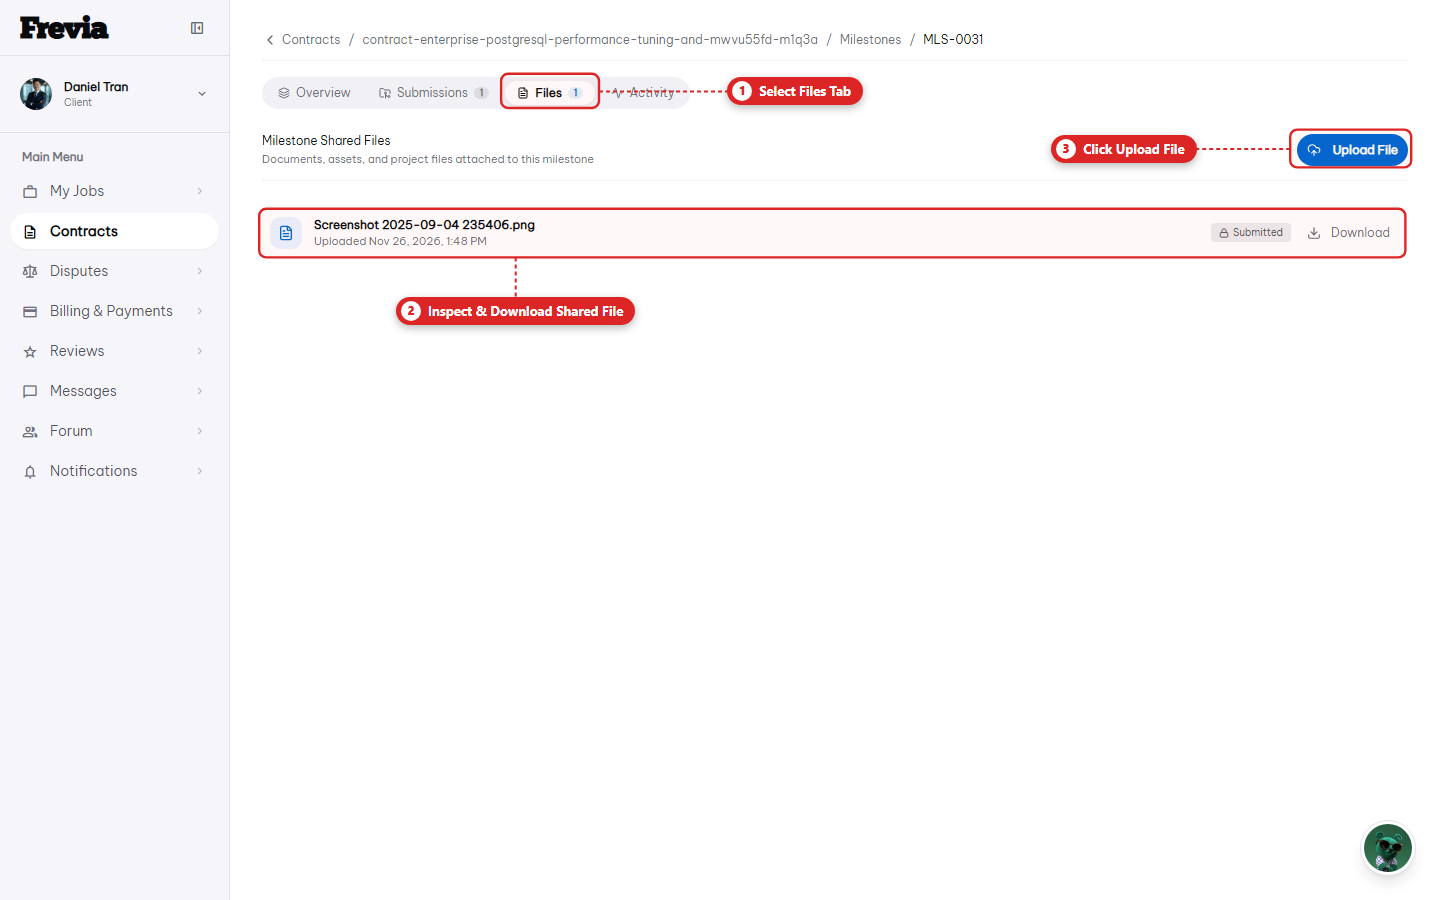
\includegraphics[width=0.90\textwidth]{images/milestones/m25_01_view_milestone_files_guide.png}
  \caption{Milestone Shared Files tab with upload action and download links}
  \label{fig:m25_01_view_milestone_files}
\end{figure}
\Needspace{6\baselineskip}\paragraph{Step-by-Step User Guide:}
\begin{enumerate}[leftmargin=1.8em,itemsep=3pt]
  \item \rbadge{1} \textbf{Select Files Tab:} Click the \textbf{Files} tab with counter badge inside Milestone Detail.
  \item \rbadge{2} \textbf{Inspect \& Download Shared File:} Review uploaded assets, upload timestamps, lock badges (e.g., \textit{Submitted}), and click \textbf{Download} to retrieve a file.
  \item \rbadge{3} \textbf{Click Upload File:} Click the blue \textbf{Upload File} button at the top right whenever you need to attach additional working assets.
\end{enumerate}
\Needspace{6\baselineskip}\paragraph{After You Submit (Result \& Troubleshooting):}
\begin{itemize}[leftmargin=1.5em,itemsep=2pt]
  \item \textbf{What Happens Next:} All files attached specifically to this milestone stage list cleanly in reverse chronological order.
  \item \textbf{Troubleshooting \& Common Messages:} Files locked inside a submitted deliverable review remain read-only until reviewed.
\end{itemize}

% -----------------------------------------------------------------------------
\newpage
\subsubsection{M25.02 -- Upload Milestone File (UC-25.02)}

\begin{itemize}[leftmargin=1.5em,itemsep=2pt]
  \item \textbf{Screen Name \& Route Path:} Milestone Files Tab -- \texttt{/[role]/\allowbreak{}contracts/\allowbreak{}[slug]/\allowbreak{}milestones/\allowbreak{}[milestoneId]}.
  \item \textbf{Target Actor:} Client, Freelancer.
  \item \Needspace{6\baselineskip}\textbf{Before You Begin:} Milestone belongs to an active contract and is currently open for collaboration.
\end{itemize}
\begin{figure}[H]\centering
  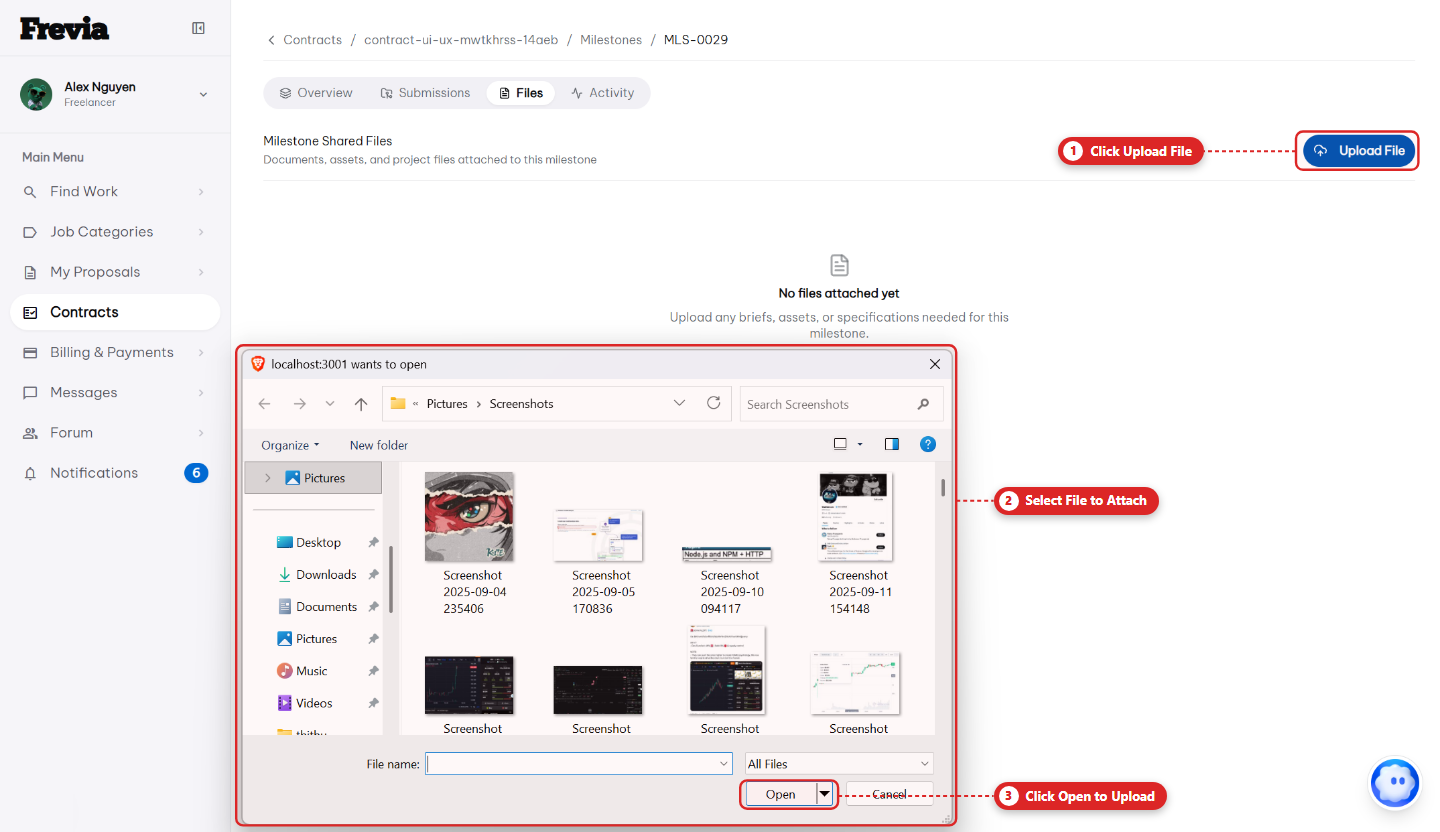
\includegraphics[width=0.90\textwidth]{images/milestones/m25_02_upload_milestone_file_guide.png}
  \caption{Uploading a milestone-specific brief or asset file from disk}
  \label{fig:m25_02_upload_milestone_file}
\end{figure}
\Needspace{6\baselineskip}\paragraph{Step-by-Step User Guide:}
\begin{enumerate}[leftmargin=1.8em,itemsep=3pt]
  \item \rbadge{1} \textbf{Click Upload File:} Inside the \textbf{Files} tab, click \textbf{Upload File}.
  \item \rbadge{2} \textbf{Select File to Attach:} Pick your asset, document, or archive in the system file chooser window.
  \item \rbadge{3} \textbf{Click Open to Upload:} Click \textbf{Open} to stream and attach the file to the milestone's \textbf{Milestone Shared Files} list.
\end{enumerate}
\Needspace{6\baselineskip}\paragraph{After You Submit (Result \& Troubleshooting):}
\begin{itemize}[leftmargin=1.5em,itemsep=2pt]
  \item \textbf{What Happens Next:} The file uploads immediately, increments the \textbf{Files} tab counter badge, and becomes downloadable by the counterparty.
  \item \textbf{Troubleshooting \& Common Messages:} Files exceeding maximum allowed size or invalid formats trigger an upload error toast.
\end{itemize}

% -----------------------------------------------------------------------------
\newpage
\subsubsection{M25.03 -- Delete Milestone File (UC-25.03)}

\begin{itemize}[leftmargin=1.5em,itemsep=2pt]
  \item \textbf{Screen Name \& Route Path:} Delete Milestone File Modal -- \texttt{/[role]/\allowbreak{}contracts/\allowbreak{}[slug]/\allowbreak{}milestones/\allowbreak{}[milestoneId]}.
  \item \textbf{Target Actor:} Uploader / Client.
  \item \Needspace{6\baselineskip}\textbf{Before You Begin:} Click the trash icon on an unlocked file entry in the milestone's \textbf{Files} tab.
\end{itemize}
\begin{figure}[H]\centering
  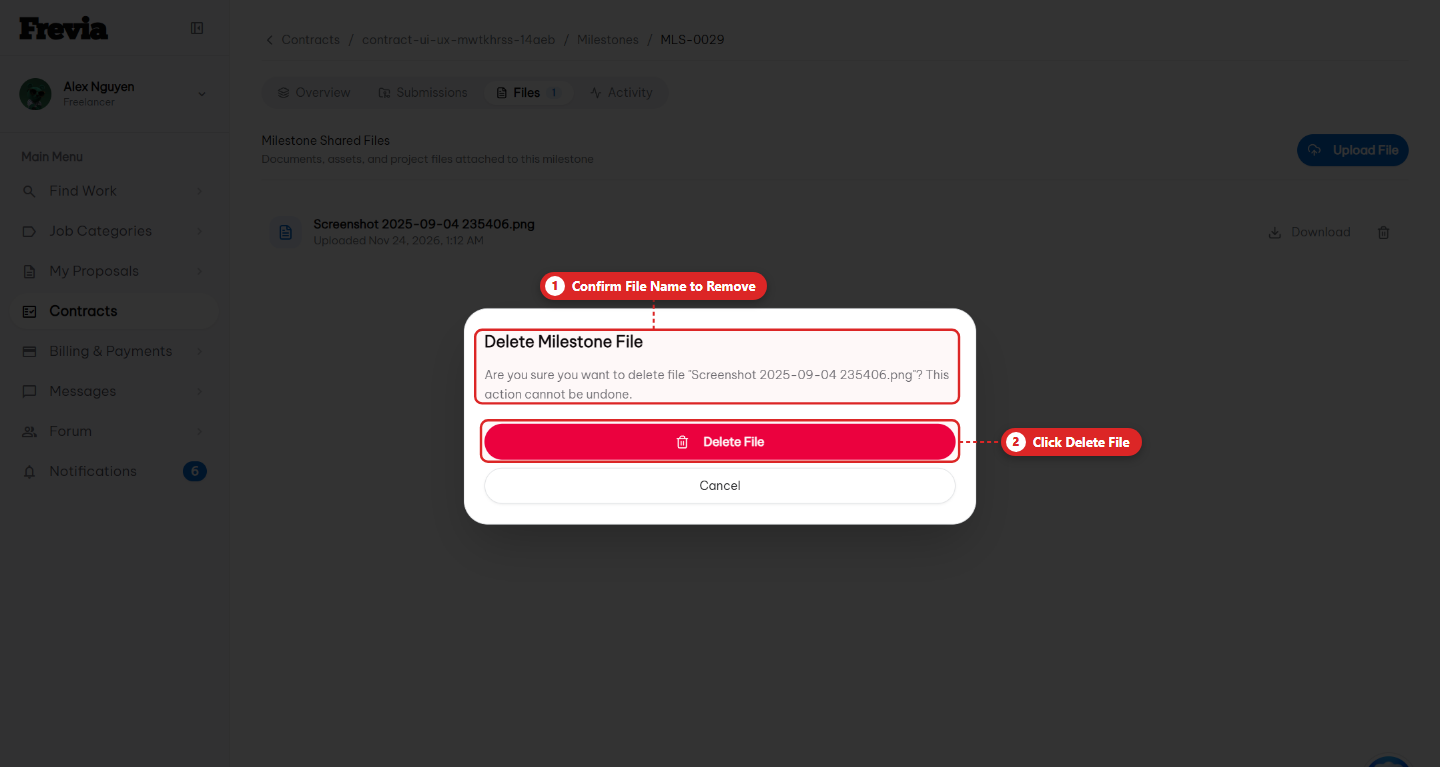
\includegraphics[width=0.90\textwidth]{images/milestones/m25_03_delete_milestone_file_guide.png}
  \caption{Delete Milestone File confirmation prompt}
  \label{fig:m25_03_delete_milestone_file}
\end{figure}
\Needspace{6\baselineskip}\paragraph{Step-by-Step User Guide:}
\begin{enumerate}[leftmargin=1.8em,itemsep=3pt]
  \item \rbadge{1} \textbf{Confirm File Name to Remove:} Read the dialog prompt verifying the filename scheduled for permanent removal.
  \item \rbadge{2} \textbf{Click Delete File:} Click the red \textbf{Delete File} button to complete removal.
\end{enumerate}
\Needspace{6\baselineskip}\paragraph{After You Submit (Result \& Troubleshooting):}
\begin{itemize}[leftmargin=1.5em,itemsep=2pt]
  \item \textbf{What Happens Next:} The file is unlinked and removed from the milestone file tray cleanly.
  \item \textbf{Troubleshooting \& Common Messages:} Files bound to submitted deliverables or active disputes cannot be deleted to preserve audit evidence.
\end{itemize}

% -----------------------------------------------------------------------------
\newpage
\subsubsection{M26.01 -- Submit Milestone Deliverable (UC-26.01)}

\begin{itemize}[leftmargin=1.5em,itemsep=2pt]
  \item \textbf{Screen Name \& Route Path:} Submit Milestone Deliverables Drawer -- \texttt{/freelancer/\allowbreak{}contracts/\allowbreak{}[slug]/\allowbreak{}milestones/\allowbreak{}[milestoneId]}.
  \item \textbf{Target Actor:} Freelancer.
  \item \Needspace{6\baselineskip}\textbf{Before You Begin:} Milestone is funded in escrow and in active/late/revision-requested state.
\end{itemize}
\begin{figure}[H]\centering
  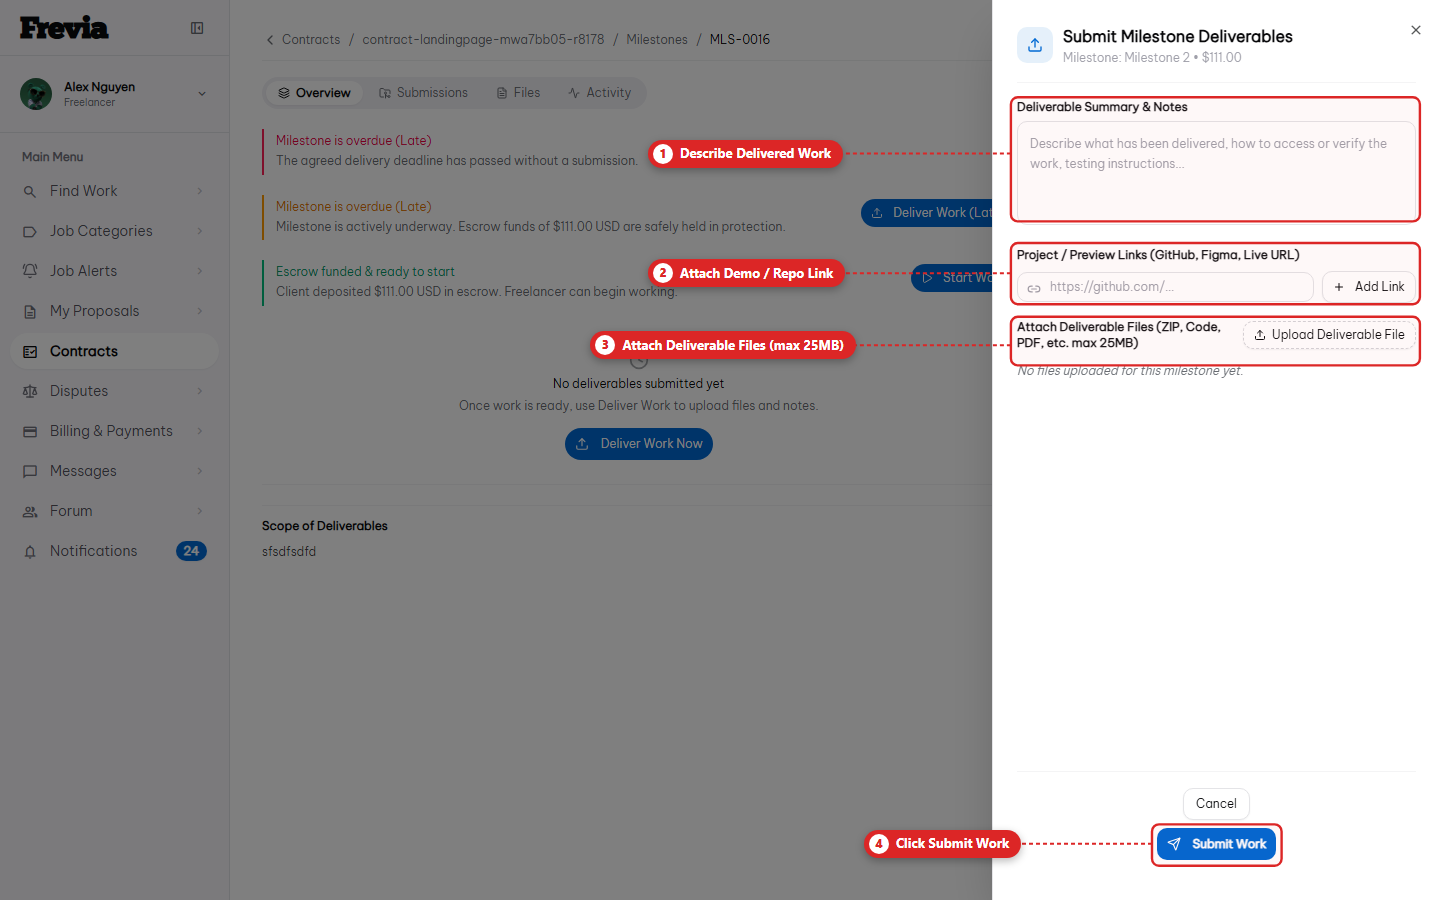
\includegraphics[width=0.90\textwidth]{images/milestones/m26_01_submit_milestone_guide.png}
  \caption{Submit Milestone Deliverables drawer with notes, demo links, and file upload}
  \label{fig:m26_01_submit_milestone}
\end{figure}
\Needspace{6\baselineskip}\paragraph{Step-by-Step User Guide:}
\begin{enumerate}[leftmargin=1.8em,itemsep=3pt]
  \item \rbadge{1} \textbf{Describe Delivered Work:} Enter testing notes, summary of completed scope, and verification guidance in \textit{Deliverable Summary \& Notes}.
  \item \rbadge{2} \textbf{Attach Demo / Repo Link:} Paste a GitHub, Figma, or staging URL and click \textbf{+ Add Link}.
  \item \rbadge{3} \textbf{Attach Deliverable Files (max 25MB):} Click \textbf{Upload Deliverable File} to attach source ZIP archives, builds, or PDF reports.
  \item \rbadge{4} \textbf{Click Submit Work:} Click \textbf{Submit Work} to transmit the formal submission for Client inspection.
\end{enumerate}
\Needspace{6\baselineskip}\paragraph{After You Submit (Result \& Troubleshooting):}
\begin{itemize}[leftmargin=1.5em,itemsep=2pt]
  \item \textbf{What Happens Next:} Milestone status changes to \texttt{SUBMITTED} (\textit{Work delivered and awaiting client review}), starting a 7-day automated approval review window.
  \item \textbf{Troubleshooting \& Common Messages:} Submitting empty notes without any links or attachments triggers a validation warning.
\end{itemize}

% -----------------------------------------------------------------------------
\newpage
\subsubsection{M26.02 -- View Milestone Submissions List (UC-26.02)}

\begin{itemize}[leftmargin=1.5em,itemsep=2pt]
  \item \textbf{Screen Name \& Route Path:} Milestone Submissions Tab -- \texttt{/[role]/\allowbreak{}contracts/\allowbreak{}[slug]/\allowbreak{}milestones/\allowbreak{}[milestoneId]}.
  \item \textbf{Target Actor:} Client, Freelancer.
  \item \Needspace{6\baselineskip}\textbf{Before You Begin:} At least one deliverable submission has been submitted for the milestone.
\end{itemize}
\begin{figure}[H]\centering
  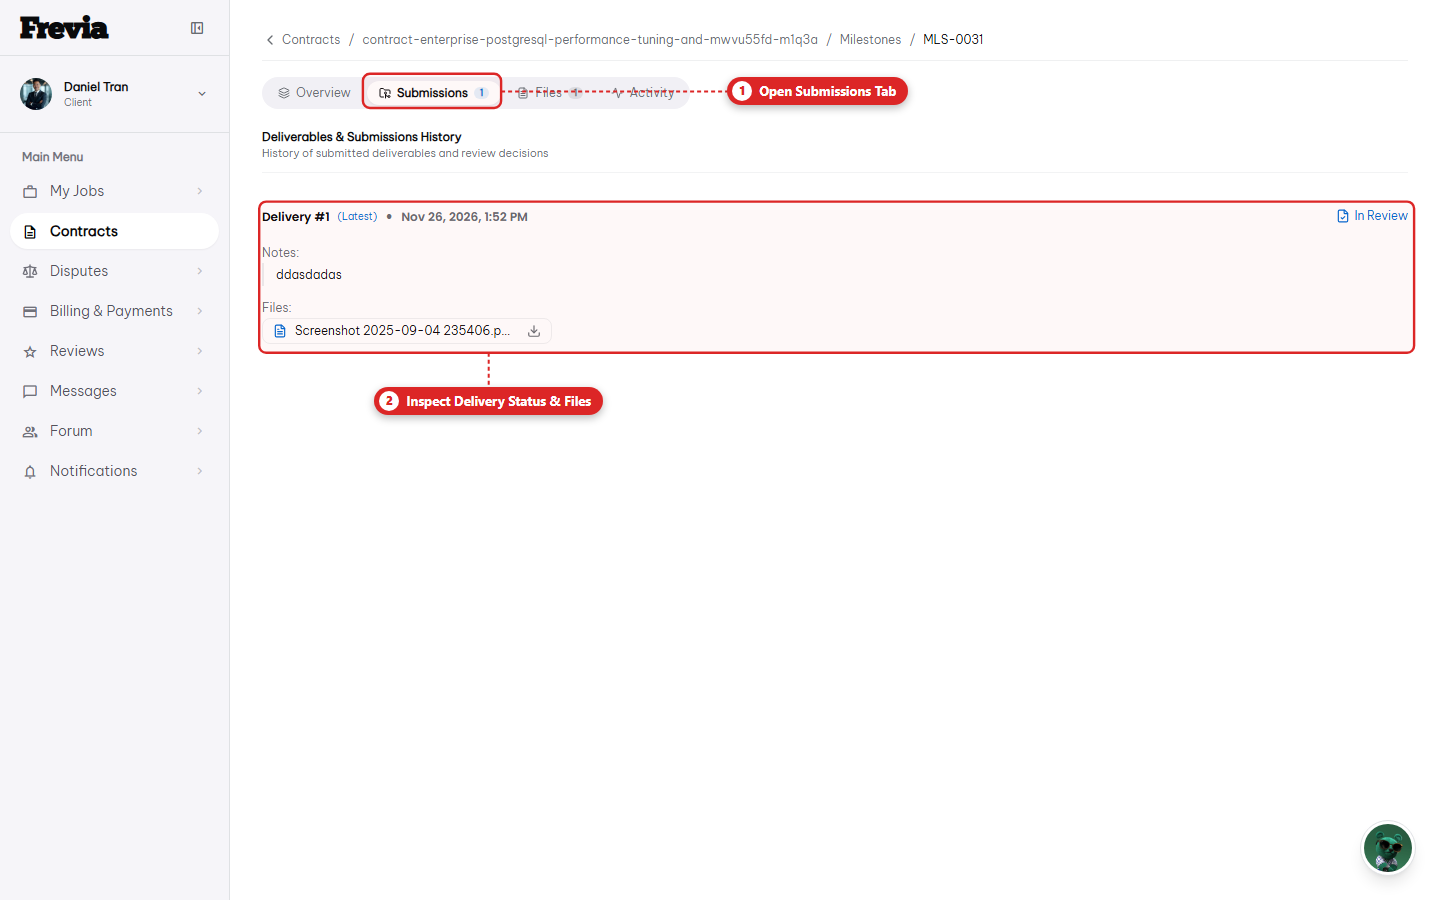
\includegraphics[width=0.90\textwidth]{images/milestones/m26_02_view_submission_list_guide.png}
  \caption{Deliverables \& Submissions History tab displaying delivery cards and status}
  \label{fig:m26_02_view_submission_list}
\end{figure}
\Needspace{6\baselineskip}\paragraph{Step-by-Step User Guide:}
\begin{enumerate}[leftmargin=1.8em,itemsep=3pt]
  \item \rbadge{1} \textbf{Open Submissions Tab:} Click \textbf{Submissions} inside the Milestone Detail tab bar.
  \item \rbadge{2} \textbf{Inspect Delivery Status \& Files:} Review chronological delivery rounds (\textit{Delivery \#1 (Latest)}), attached files, freelancer notes, and status pills (\textit{In Review}, \textit{Revision Requested}, or \textit{Approved}).
\end{enumerate}
\Needspace{6\baselineskip}\paragraph{After You Submit (Result \& Troubleshooting):}
\begin{itemize}[leftmargin=1.5em,itemsep=2pt]
  \item \textbf{What Happens Next:} Every historical submission round and client review decision remains auditable in one timeline.
  \item \textbf{Troubleshooting \& Common Messages:} Before the first delivery, an informational banner notes no deliverables have been submitted yet.
\end{itemize}

% -----------------------------------------------------------------------------
\newpage
\subsubsection{M26.03 -- View Milestone Submission Details (UC-26.03)}

\begin{itemize}[leftmargin=1.5em,itemsep=2pt]
  \item \textbf{Screen Name \& Route Path:} Review Work Submission Drawer -- \texttt{/client/\allowbreak{}contracts/\allowbreak{}[slug]/\allowbreak{}milestones/\allowbreak{}[milestoneId]}.
  \item \textbf{Target Actor:} Client, Freelancer.
  \item \Needspace{6\baselineskip}\textbf{Before You Begin:} Click \textbf{Review \& Approve Delivery} on a delivered milestone's Overview or Submissions tab.
\end{itemize}
\begin{figure}[H]\centering
  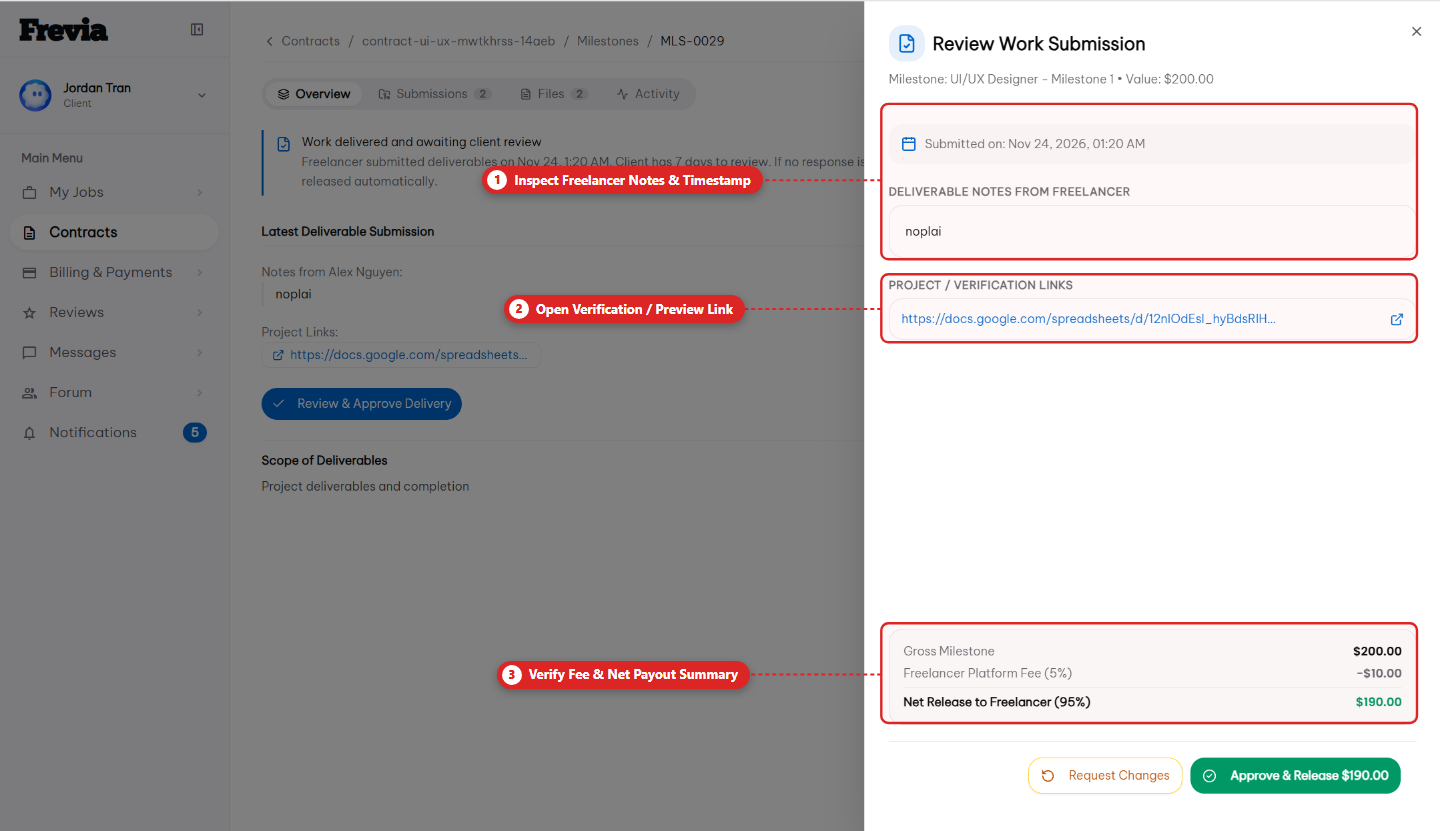
\includegraphics[width=0.90\textwidth]{images/milestones/m26_03_view_submission_detail_guide.png}
  \caption{Review Work Submission drawer detailing notes, verification links, and fee split}
  \label{fig:m26_03_view_submission_detail}
\end{figure}
\Needspace{6\baselineskip}\paragraph{Step-by-Step User Guide:}
\begin{enumerate}[leftmargin=1.8em,itemsep=3pt]
  \item \rbadge{1} \textbf{Inspect Freelancer Notes \& Timestamp:} Verify exact delivery timestamp and notes explaining implementation and testing details.
  \item \rbadge{2} \textbf{Open Verification / Preview Link:} Click external project links or download attached archive files to inspect deliverables thoroughly.
  \item \rbadge{3} \textbf{Verify Fee \& Net Payout Summary:} Confirm gross milestone value, 5\% platform fee deduction, and exact net release to the Freelancer.
\end{enumerate}
\Needspace{6\baselineskip}\paragraph{After You Submit (Result \& Troubleshooting):}
\begin{itemize}[leftmargin=1.5em,itemsep=2pt]
  \item \textbf{What Happens Next:} You can immediately decide between requesting targeted changes (\textbf{M26.04}) or approving and releasing escrow funds (\textbf{M26.05}).
  \item \textbf{Troubleshooting \& Common Messages:} Expired 7-day unreviewed submissions auto-approve cleanly via scheduled escrow automation.
\end{itemize}

% -----------------------------------------------------------------------------
\newpage
\subsubsection{M26.04 -- Request Milestone Changes (UC-26.04)}

\begin{itemize}[leftmargin=1.5em,itemsep=2pt]
  \item \textbf{Screen Name \& Route Path:} Review Work Submission (Revision Mode) -- \texttt{/client/\allowbreak{}contracts/\allowbreak{}[slug]/\allowbreak{}milestones/\allowbreak{}[milestoneId]}.
  \item \textbf{Target Actor:} Client.
  \item \Needspace{6\baselineskip}\textbf{Before You Begin:} Inside the \textbf{Review Work Submission} drawer, click \textbf{Request Changes}.
\end{itemize}
\begin{figure}[H]\centering
  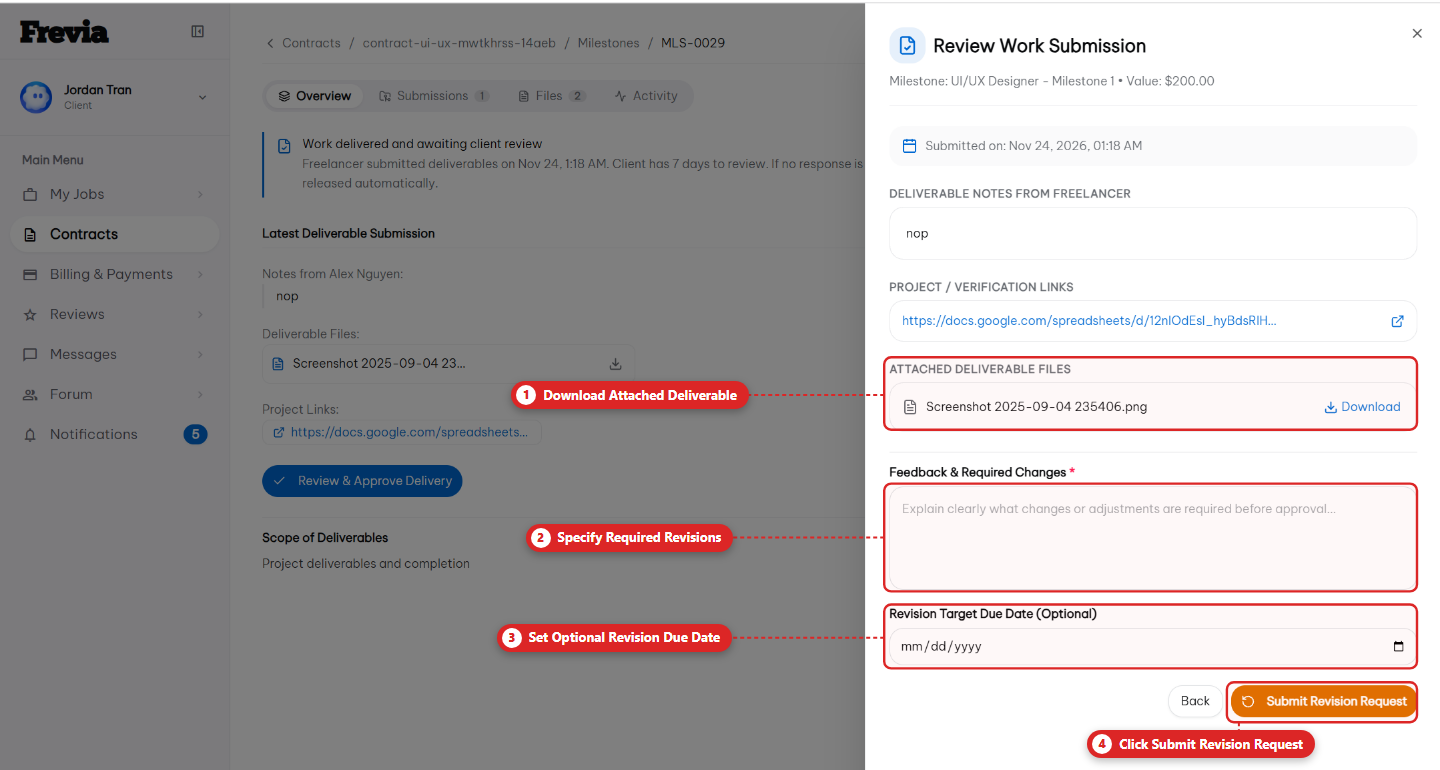
\includegraphics[width=0.90\textwidth]{images/milestones/m26_04_request_milestone_changes_guide.png}
  \caption{Requesting deliverable revisions with structured feedback and target due date}
  \label{fig:m26_04_request_milestone_changes}
\end{figure}
\Needspace{6\baselineskip}\paragraph{Step-by-Step User Guide:}
\begin{enumerate}[leftmargin=1.8em,itemsep=3pt]
  \item \rbadge{1} \textbf{Download Attached Deliverable:} Reference any attached submission files directly while writing feedback.
  \item \rbadge{2} \textbf{Specify Required Revisions:} Enter clear, actionable adjustments required before approval in \textit{Feedback \& Required Changes *}.
  \item \rbadge{3} \textbf{Set Optional Revision Due Date:} Optionally specify a new revision target deadline.
  \item \rbadge{4} \textbf{Click Submit Revision Request:} Click the amber \textbf{Submit Revision Request} button to return the milestone to the Freelancer.
\end{enumerate}
\Needspace{6\baselineskip}\paragraph{After You Submit (Result \& Troubleshooting):}
\begin{itemize}[leftmargin=1.5em,itemsep=2pt]
  \item \textbf{What Happens Next:} Escrow remains safely held, the milestone transitions to revision requested, and the Freelancer is notified to submit an updated delivery.
  \item \textbf{Troubleshooting \& Common Messages:} Submitting without written revision feedback triggers client-side required field validation.
\end{itemize}

% -----------------------------------------------------------------------------
\newpage
\subsubsection{M26.05 -- Approve Milestone Deliverable (UC-26.05)}

\begin{itemize}[leftmargin=1.5em,itemsep=2pt]
  \item \textbf{Screen Name \& Route Path:} Review Work Submission Drawer -- \texttt{/client/\allowbreak{}contracts/\allowbreak{}[slug]/\allowbreak{}milestones/\allowbreak{}[milestoneId]}.
  \item \textbf{Target Actor:} Client.
  \item \Needspace{6\baselineskip}\textbf{Before You Begin:} Milestone is in \texttt{SUBMITTED} state after Freelancer deliverable submission.
\end{itemize}
\begin{figure}[H]\centering
  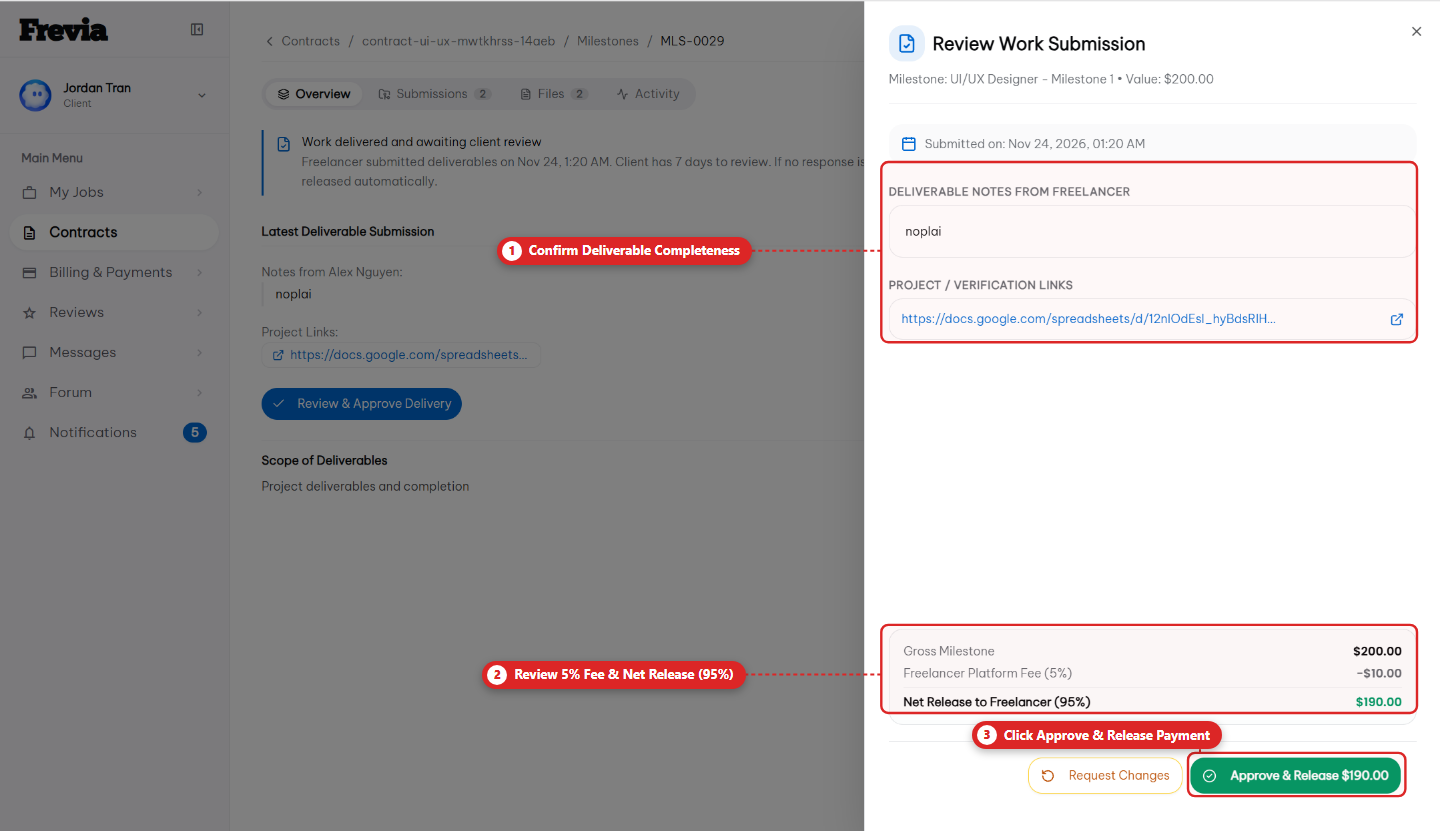
\includegraphics[width=0.90\textwidth]{images/milestones/m26_05_approve_milestone_guide.png}
  \caption{Approve \& Release deliverable confirmation inside Review Work Submission}
  \label{fig:m26_05_approve_milestone}
\end{figure}
\Needspace{6\baselineskip}\paragraph{Step-by-Step User Guide:}
\begin{enumerate}[leftmargin=1.8em,itemsep=3pt]
  \item \rbadge{1} \textbf{Confirm Deliverable Completeness:} Verify submitted notes, links, and attached work satisfy milestone scope.
  \item \rbadge{2} \textbf{Review 5\% Fee \& Net Release (95\%):} Check the calculated net payout (95\% of gross milestone value) that will transfer via Stripe Connect.
  \item \rbadge{3} \textbf{Click Approve \& Release Payment:} Click the green \textbf{Approve \& Release} button to accept the delivery and trigger payout release.
\end{enumerate}
\Needspace{6\baselineskip}\paragraph{After You Submit (Result \& Troubleshooting):}
\begin{itemize}[leftmargin=1.5em,itemsep=2pt]
  \item \textbf{What Happens Next:} The submission and milestone transition to \texttt{APPROVED}/\texttt{COMPLETED}, Stripe transfers net funds to the Freelancer, and contract progress updates automatically.
  \item \textbf{Troubleshooting \& Common Messages:} If the Freelancer has not completed Stripe Connect Express payouts setup, the system prompts onboarding completion before final transfer.
\end{itemize}
